\begin{equation}
    \begin{gathered}
        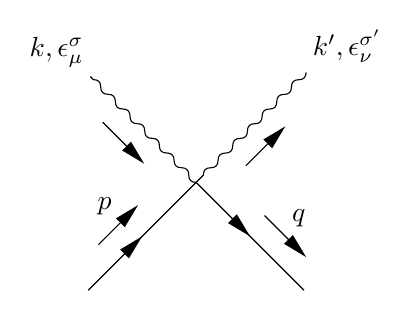
\begin{tikzpicture}[x=0.75pt,y=0.75pt,yscale=-1,xscale=1]
            %uncomment if require: \path (0,300); %set diagram left start at 0, and has height of 300
            
            %Straight Lines [id:da1122667009577647] 
            \draw    (236,132) .. controls (236,134.36) and (234.82,135.54) .. (232.46,135.54) .. controls (230.11,135.54) and (228.93,136.72) .. (228.93,139.07) .. controls (228.93,141.43) and (227.75,142.61) .. (225.39,142.61) .. controls (223.04,142.61) and (221.86,143.79) .. (221.86,146.14) .. controls (221.86,148.5) and (220.68,149.68) .. (218.32,149.68) .. controls (215.97,149.68) and (214.79,150.86) .. (214.79,153.21) .. controls (214.79,155.57) and (213.61,156.75) .. (211.25,156.75) .. controls (208.9,156.75) and (207.72,157.93) .. (207.72,160.28) .. controls (207.72,162.64) and (206.54,163.82) .. (204.18,163.82) .. controls (201.82,163.82) and (200.64,165) .. (200.64,167.36) .. controls (200.64,169.71) and (199.46,170.89) .. (197.11,170.89) .. controls (194.75,170.89) and (193.57,172.07) .. (193.57,174.43) .. controls (193.57,176.78) and (192.39,177.96) .. (190.04,177.96) .. controls (187.68,177.96) and (186.5,179.14) .. (186.5,181.5) -- (183,185) -- (183,185) ;
            %Straight Lines [id:da6518370903341117] 
            \draw    (183,185) .. controls (180.64,185) and (179.46,183.82) .. (179.46,181.46) .. controls (179.46,179.11) and (178.28,177.93) .. (175.93,177.93) .. controls (173.57,177.93) and (172.39,176.75) .. (172.39,174.39) .. controls (172.39,172.04) and (171.21,170.86) .. (168.86,170.86) .. controls (166.5,170.86) and (165.32,169.68) .. (165.32,167.32) .. controls (165.32,164.97) and (164.14,163.79) .. (161.79,163.79) .. controls (159.43,163.79) and (158.25,162.61) .. (158.25,160.25) .. controls (158.25,157.9) and (157.07,156.72) .. (154.72,156.72) .. controls (152.36,156.72) and (151.18,155.54) .. (151.18,153.18) .. controls (151.18,150.82) and (150,149.64) .. (147.64,149.64) .. controls (145.29,149.64) and (144.11,148.46) .. (144.11,146.11) .. controls (144.11,143.75) and (142.93,142.57) .. (140.57,142.57) .. controls (138.22,142.57) and (137.04,141.39) .. (137.04,139.04) .. controls (137.04,136.68) and (135.86,135.5) .. (133.5,135.5) -- (132,134) -- (132,134) ;
            %Straight Lines [id:da7053680489481458] 
            \draw    (183,185) -- (235,237) ;
            \draw [shift={(209,211)}, rotate = 225] [fill={rgb, 255:red, 0; green, 0; blue, 0 }  ][line width=0.08]  [draw opacity=0] (12,-3) -- (0,0) -- (12,3) -- cycle    ;
            %Straight Lines [id:da34290471930097643] 
            \draw    (131,237) -- (183,185) ;
            \draw [shift={(157,211)}, rotate = 135] [fill={rgb, 255:red, 0; green, 0; blue, 0 }  ][line width=0.08]  [draw opacity=0] (12,-3) -- (0,0) -- (12,3) -- cycle    ;
            %Straight Lines [id:da08502578298763375] 
            \draw    (216,201) -- (234.59,219.59) ;
            \draw [shift={(236,221)}, rotate = 225] [fill={rgb, 255:red, 0; green, 0; blue, 0 }  ][line width=0.08]  [draw opacity=0] (12,-3) -- (0,0) -- (12,3) -- cycle    ;
            %Straight Lines [id:da33302439344255874] 
            \draw    (136,215) -- (153.59,197.41) ;
            \draw [shift={(155,196)}, rotate = 135] [fill={rgb, 255:red, 0; green, 0; blue, 0 }  ][line width=0.08]  [draw opacity=0] (12,-3) -- (0,0) -- (12,3) -- cycle    ;
            %Straight Lines [id:da13456778366163258] 
            \draw    (207,177) -- (224.59,159.41) ;
            \draw [shift={(226,158)}, rotate = 135] [fill={rgb, 255:red, 0; green, 0; blue, 0 }  ][line width=0.08]  [draw opacity=0] (12,-3) -- (0,0) -- (12,3) -- cycle    ;
            %Straight Lines [id:da5790372952068077] 
            \draw    (138,156) -- (156.59,174.59) ;
            \draw [shift={(158,176)}, rotate = 225] [fill={rgb, 255:red, 0; green, 0; blue, 0 }  ][line width=0.08]  [draw opacity=0] (12,-3) -- (0,0) -- (12,3) -- cycle    ;
            
            % Text Node
            \draw (130,130.6) node [anchor=south east] [inner sep=0.75pt]    {$k,\epsilon _{\mu }^{\sigma }$};
            % Text Node
            \draw (238,128.6) node [anchor=south west] [inner sep=0.75pt]    {$k',\epsilon _{\nu }^{\sigma '}$};
            % Text Node
            \draw (143.5,202.1) node [anchor=south east] [inner sep=0.75pt]    {$p$};
            % Text Node
            \draw (228,207.6) node [anchor=south west] [inner sep=0.75pt]    {$q$};
            \end{tikzpicture}            
    \end{gathered} = (\epsilon^\sigma)^\mu (\epsilon^{\sigma'})^\nu \times 2 \ii e^2 \eta_{\mu \nu} \eqqcolon \ii \mathcal{M}_4,
\end{equation}